\startchapter{Least Squares Localization by Sequential Convex Relaxation}
\label{chapter:scp}

%\textbf{Notes for further development.}
%
%2-step approach:
%
%1) identify outliers to reduce the error-prone data points
%
%2) apply the algorithm  to the redused data set
%
%Projection onto convex sets and projection onto rings \textit{cite GhStr}

%\section{Second Order Cone Programming}

In connection with the problem of localizing a single radiating source based on range and range-difference measurements, in this chapter
we study the 

we convert the unconstrained least squares (LS) formulation to a constrained problem and 
we study the application of the sequential convex programming approaches


 we explore special structure of the cost function of an unconstrained least squares (LS) formulation and show that it is well suited in a setting known as ... Our focus in this chapter will be placed on the localization problem based on ... measurements.

 %We present an algorithm for solving the LS problem at hand based on a penalty convex-concave procedure (PCCP) \cite{LBoyd} that accommodates infeasible initial points in solving a fairly large class of \textit{nonconvex} constrained problems. Algorithmic details are provided to show that the PCCP-based formulation is tailored to the localization problem at hand. These include additional constraints that enforce the algorithms iteration path towards the LS solution, and several strate321q223wgies to secure good initial points. Numerical results are presented to demonstrate that the proposed algorithm offers substantial performance improvement relative to some best known results from the literature.



\section{Range-Difference Localization}
\subsection{Problem Formulation}


In this section we focus on the problem of range-difference based localization given the time-difference of arrival information. TDOA localization, also known as multilateration, or hyperbolic positioning, is a method where the position of the mobile unit (signal source) can be determined using the differences in the TOAs from different base stations. By using this method the clock biases between the mobile units and base stations are automatically removed, since only the pairwise differences between the TOAs from base stations are  considered \cite{LocAlg}.  A hyperbola is the basis for solving multilateration problems. In particular, the set of possible positions of a mobile unit that has a range difference of $d_i$ from two given base stations $BS_i$ and $BS_0$, placed at $\Ba_i$ and $\Ba_0$ respectively, is a hyperbola with vertex separation of $d_i$ and focii located at $\Ba_i$ and $\Ba_0$. $BS_0$ is placed at the origin of the coordinate system, i.e. $\Ba_0 = \symb{0}_n$, and used as a reference station. Consider now a third base station $BS_j$ at a third location. This would provide one extra independent  measurement between $BS_j$ and $BS_0$ and the source is located on the curve determined by the two intersecting hyperboloids. Figure \ref{fig:tdoa} illustrates an example of the range-difference localization based on TDOA measurements.

 \phantom{m}

\begin{figure*}[h]
\centering
%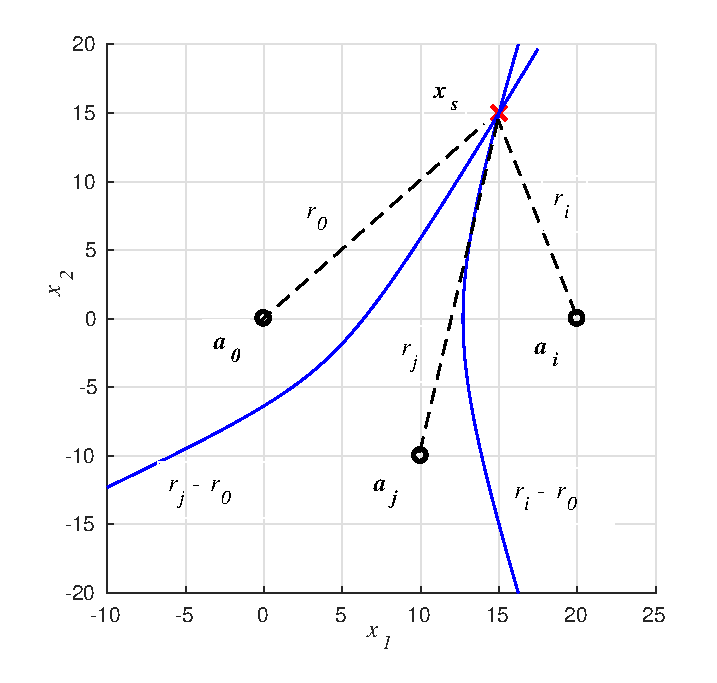
\includegraphics[height=0.45\textheight]{figures/socp_rd/TDOA_example}
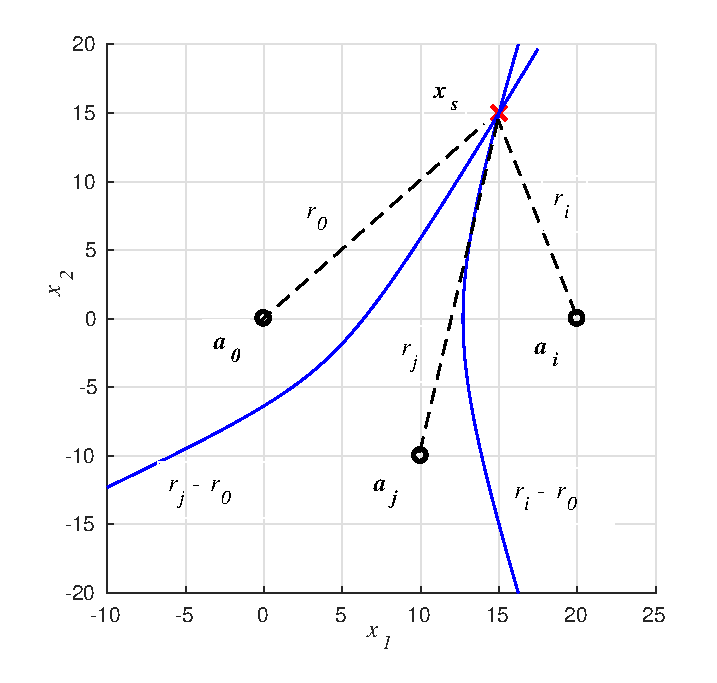
\includegraphics{figures/socp_rd/TDOA_example}
\caption{Range-difference localization.  At least three base stations are required for the planar localization. The red cross indicates the location of the signal source. Sensors are placed at $\protect\Ba_j = (10, -10)^T$, and  $\protect\Ba_0$ is the reference sensor. The time (range) differences $r_j - r_0$ and $r_i - r_0$ form two hyperboloids with focii located at $\protect\Ba_i, \protect\Ba_j$ and $\protect\Ba_0$. Note that the hyperboloids are actually double sheeted, but for visual clarity only the halves which are part of the solution are shown. The intersection of these hyperboloids is the estimated position.
The figure depicts the locus of possible source locations as one half of a two-sheeted hyperboloids.}
\label{fig:tdoa}
\end{figure*}

 \phantom{m}
%An example of location estimation using TDOA is shown in Figure \ref{fig:hyperbola}. Consider an instance of the source localization problem on the plane $n = 2$ with the reference sensor $\Ba_0$ placed at the origin and five sensors $m = 5$ located at 
%\begin{equation}
%\nonumber
%\Ba_1 = \begin{bmatrix}
%-5 \\ -13
%\end{bmatrix}, \
%\Ba_2 = \begin{bmatrix}
%-12 \\ 1
%\end{bmatrix},  \
%\Ba_3 = \begin{bmatrix}
%-1 \\ -5
%\end{bmatrix}, \
%\Ba_4 = \begin{bmatrix}
%-9 \\ -12
%\end{bmatrix}, \
%\Ba_5 = \begin{bmatrix}
%-3 \\ -12
%\end{bmatrix}
%\\
%\end{equation}
%
%The source emitting the signal was located at $\Bx_s = (-5,11)^T$. Figure \ref{fig:hyperbola} depicts the locus of possible source locations as one half of a two-sheeted hyperboloids.

%\begin{figure} 
%\centering
%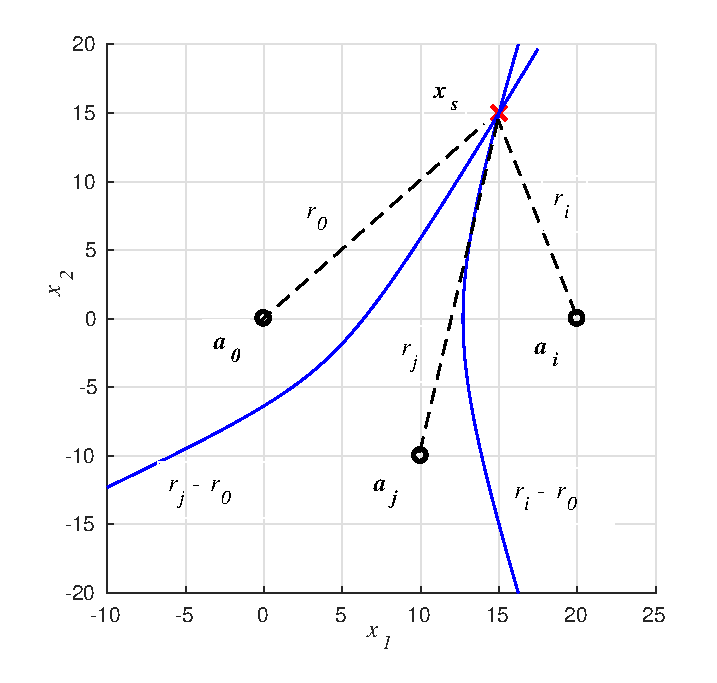
\includegraphics{figures/socp_rd/TDOA_example}
%\caption{Algorithm and contours of the R-LS objective function over the region $\protect\Re = \protect\lbrace \protect\Bx:-15\protect\leq x_1 \protect\leq 15, -25\protect\leq x_2 \protect\leq 15 \protect\rbrace$. The red cross indicates the location of the signal source. Sensors are located at $(-5, -13)^T$, $(-12, 1)^T$, $(-1, -5)^T$, $(-9, -12)^T$ and  $(-3, -12)^T$. Hyperbolas denote possible source locations given the pairwise range-difference readings. Large circles denote possible source locations given the noisy range reading at a particular sensor.}
%\label{fig:hyperbola}
%\end{figure}
 
%Given two base station locations $BS_i$ and $BS_0$, placed at $\Ba_i$ and $\Ba_0$ respectively, with $BS_0$ placed at the origin of the coordinate system, i.e. $\Ba_0 = \symb{0}_n$, and used as a reference station, and a known TDOA, the locus of possible source locations is one half of a two-sheeted hyperboloid. Consider now a third base station $BS_j$ at a third location. This would provide one extra independed TDOA measurement and the source is located on the curve determined by the two intersecting hyperboloids.

%Each TDOA measurement constrains the location of the signal source to be on a hyperboloid with a constant range-difference between the two reference points.

%\textit{Matlab} Using the arrival times, the time differences of arrival between each pair of eNodeBs is calculated using hPositioningTDOA.m. The particular time difference of arrival between a pair of eNodeBs can result from the UE being located at any position where two circles, each centered on an eNodeB, intersect. The two circles have radii which differ by the distance covered at the speed of light in the given time difference. The complete set of possible UE positions across all possible radii for one circle (with the other circle maintaining a radius appropriate to the time difference as already described) forms a hyperbola. The "hyperbolas of constant delay difference" for all the different pairs of eNodeBs are plotted relative to the known eNodeB positions and intersect at the position of the UE.
%A hyperbola is the basis for solving multilateration problems, the task of locating a point from the differences in its distances to given points — or, equivalently, the difference in arrival times of synchronized signals between the point and the given points. Such problems are important in navigation, particularly on water; a ship can locate its position from the difference in arrival times of signals from a LORAN or GPS transmitters. Conversely, a homing beacon or any transmitter can be located by comparing the arrival times of its signals at two separate receiving stations; such techniques may be used to track objects and people. In particular, the set of possible positions of a point that has a distance difference of 2a from two given points is a hyperbola of vertex separation 2a whose foci are the two given points.

%\textit{Wiki} If a pulse is emitted from a platform, it will generally arrive at slightly different times at two spatially separated receiver sites, the TDOA being due to the different distances of each receiver from the platform. In fact, for given locations of the two receivers, a whole set of emitter locations would give the same measurement of TDOA. Given two receiver locations and a known TDOA, the locus of possible emitter locations is one half of a two-sheeted hyperboloid.

%\textit{Wiki} In simple terms, with two receivers at known locations, an emitter can be located onto a hyperboloid.[1] Note that the receivers do not need to know the absolute time at which the pulse was transmitted – only the time difference is needed. A fourth receiver is needed for another independed TDOA, this wil give an extra hyperboloid, the intersection of the curve with this hyperboloid gives one or two solutions, the emitter is then located at the one or at the one of the two solutions.



The localization problem discussed in this section involves a given array of $m+1$ sensors placed in the $n = 2$ or 3 dimentional space with coordinates specified by $\{\Ba_1, \Ba_2, . . . , \Ba_m , a_i \in R^n\}$ and  $\Ba_0 = \symb{0}_n$ placed at the origin and used as a refference sensor. The localization problem here is to estimate the location of a radiating source $\Bx$ given the locations of the $m+1$ sensors and noise-contaminated range-difference measurements $\{d_i, i = 1, 2, \ldots, m\}$ where 
\setcounter{abc}{0}
\begin{equation} \label{eq:6.1}
d_i = \|\Bx - \Ba_i\| - \|\Bx\| + \varepsilon_i, \mbox{ for } i = 1, 2, \ldots, m
\end{equation}
Therefore, the standard range-difference LS (RD-LS) problem is formulated as
\begin{equation} \label{eq:6.2}
\Min \sum^m_{i=1}\left( \|\Bx - \Ba_i\| - \|\Bx\| - d_i\right)^2
\end{equation}
As described in Sec.2.2 of the thesis, finding the solution to ($\ref{eq:6.2}$) is a non-trivial problem and many approaches have been developed to address this problem. In the following we propose a new iterative procedure to tackle the RD-LS problem (\ref{eq:6.2}), with the goal of achieving a more accurate and robust solution. The central part of the procedure is a convex quadratic programming (QP) problem that needs to be solved in each iteration to provide an increment vector that updates the present iterate to next towards the solution of the localization problem at hand.

\subsection{Sequential Convex Relaxation}

%\newpage 
%
%\input chapters/5/scp_rd_ls
%
%\newpage

We begin by re-writing the unconstrained problem in (\ref{eq:6.2}) as a constrained problem with second-order cone constraints%can be equivalently written as
\setcounter{abc}{0}
\begin{eqnarray} \label{eq:6.3} %1.7
\stepcounter{abc}
\setcounter{equation}{3}
\Min_{\Bx, y, \Bz} & & \sum^m_{i=1}\left( z_i - y - d_i\right)^2\\
\stepcounter{abc}
\setcounter{equation}{3}
\mbox{subject to:}& &\|\Bx - \Ba_i\| = z_i \\
\stepcounter{abc}
\setcounter{equation}{3}
& &\|\Bx\|  = y, \quad  i = 1, 2, \ldots m
\end{eqnarray}
Assume we are in the $k$th iteration and we are to update the $k$th iterate $\{\Bx_k,y_k,\Bz_k\}$. Let the next iterate be
\setcounter{abc}{0}
\begin{eqnarray} \label{eq:6.4} %1.8
\stepcounter{abc}
\Bx^{k+1} &=& \Bx^k + \Bdelta_x \\
\stepcounter{abc}
\setcounter{equation}{4}
y^{k+1} &=& y^k + \delta_y \\
\stepcounter{abc}
\setcounter{equation}{4}
\Bz^{k+1} &=& \Bz^k + \Bdelta_z
\end{eqnarray}
where $\{\Bdelta_x, \delta_y, \Bdelta_z\}$ are such that the constraints in (\ref{eq:6.3}b) and (\ref{eq:6.3}c) are better approximated at $\{\Bx_{k+1},y_{k+1},\Bz_{k+1}\}$ in the sense that
\setcounter{abc}{0}
\begin{eqnarray}
\nonumber
\|\Bx_{k+1} - \Ba_i\| &\approx &z_i^{k+1}, \quad i = 1, 2, \ldots, m \\
\nonumber
\|\Bx_{k+1}\| &\approx &y_{k+1}
\end{eqnarray}
namely,
\setcounter{abc}{0}
\begin{eqnarray}
\nonumber
\|\Bx_{k} + \Bdelta_x - \Ba_i\| &\approx &z_i^{k} + \Bdelta_{z_i}, \quad i = 1, 2, \ldots, m \\
\nonumber
\|\Bx_{k} + \Bdelta_x\| &\approx &y_{k}  + \Bdelta_y
\end{eqnarray}
By replacing the left-hand sides of the above equations with their first-order Taylor approximations, we obtain
\setcounter{abc}{0}
\begin{eqnarray}
\nonumber
\|\Bx_{k} - \Ba_i\| + \partial_x^T\|\Bx_{k} - \Ba_i\|\Bdelta_x &\approx & z_i^{k} + \Bdelta_{z_i}, \quad i = 1, 2, \ldots, m \\
\nonumber
\|\Bx_{k}\|  + \partial_x^T\|\Bx_{k}\|\Bdelta_x\ &\approx & y_{k}  + \Bdelta_y
\end{eqnarray}
where $\partial_x$ is the subdifferential operator with respect to variable $\Bx$. Assuming $\Bx_k \neq \Ba_i$ and $\Bx_k$ is nonzero, then
\begin{equation}
\nonumber
\partial_x\|\Bx_{k} - \Ba_i\| = \frac{\Be}{\|\Bx_{k} - \Ba_i\|} \ \mbox{and } \partial_x\|\Bx_{k}\| = \frac{\Be}{\|\Bx_{k}\|}
\end{equation}
where $\Be$ is the all-one vector. Hence
\setcounter{abc}{0}
\begin{eqnarray} \label{eq:6.5} %1.9
\stepcounter{abc}
\|\Bx_k - \Ba_i\| + \frac{\Be^T\Bdelta_x}{\|\Bx_k\|} &\approx &z^{(k)}_i + \delta_{z_{j}}, \quad i = 1, 2,...,m \\
\stepcounter{abc}
\setcounter{equation}{5}
\|\Bx_k\| + \frac{\Be^T\Bdelta_x}{\|\Bx_k\|} &\approx &y_k + \delta_y
\end{eqnarray}
The objective in \ref{eq:6.3} can be written as
 \setcounter{abc}{0}
\begin{eqnarray} 
\nonumber
F(\Bx_{k+1}) & =  & \sum^m_{i = 1} \left(z^{(k)}_i + \delta_{z_i} - (y_k + \delta_y) - d_i \right)^2 \\
\nonumber
& = & \sum^m_{i = 1} \left(- \delta_y + \delta_{z_i}  - \tilde{d_i^{(k)}} \right)^2
\end{eqnarray}
where 
\begin{equation}
\nonumber
\tilde{d}^{(k)}_i =  d_i - y_k - z_i^{(k)}
\end{equation}
are grouped known constant terms. Based on the above, the problem to be solved in the \textit{k}th iteration is formulated as
\setcounter{abc}{0}
\begin{eqnarray} \label{eq:6.6} %1.10
\stepcounter{abc}
\Min_{\Bdelta}& &f(\tilde{\Bdelta}) = \sum^m_{i=1}\left(-\delta_y + \delta_{z_{j}} - \tilde{d^{(k)}_i}\right)^2\\
\stepcounter{abc}
\setcounter{equation}{6}
\mbox{subject to:}& &\|\Bx_k - \Ba_i\| + \frac{\Be^T\Bdelta_x}{\|\Bx_k - \Ba_i\| } = z_i^{(k)} + \delta_{z_{j}}, i = 1, 2,...,m \\
\stepcounter{abc}
\setcounter{equation}{6}
& &\|\Bx_k\| + \frac{\Be^T\Bdelta_x}{\|\Bx_k\|} = y_k + \delta_y \\
\stepcounter{abc}
\setcounter{equation}{6}
& &\begin{bmatrix}
-\beta\BOne_2 \\
-\mbox{min}\{\beta, y_k\} \\
-\mbox{min}\{\beta, \Bz_k\}
\end{bmatrix} \leq \begin{bmatrix}
\Bdelta_x \\
\delta_y \\
\Bdelta_z
\end{bmatrix} \leq \begin{bmatrix}
\beta\BOne_2 \\
\beta \\
\beta\BOne_m
\end{bmatrix}
\end{eqnarray}
The constraints in (\ref{eq:6.6}d) not only assure that the magnitude of each component in $\{\Bdelta_x, \delta_y, \Bdelta_z\}$ is no greater than $\beta$, but also they assure that all components of $\{y_{k + 1}, \Bz_{k + 1}\}$ are nonnegative as long as $\{y_{k}, \Bz_{k}\}$ are nonnegative, which are natural to impose as can be seen from (\ref{eq:6.3}b) and (\ref{eq:6.3}c) because they are vector norms. Obviously, the problem in (\ref{eq:6.6}) is a convex QP problem. One
technical difficulty that may occur in solving problem (\ref{eq:6.6}) is that the feasible region defined by (\ref{eq:6.6}b), (\ref{eq:6.6}c), and (\ref{eq:6.6}d) may be empty. In such a case the constraints in problem (\ref{eq:6.6})
much be adequately relaxed in order for the problem to be solvable. To this end we rewrite (\ref{eq:6.6}) as
\setcounter{abc}{0}
\begin{eqnarray} \label{eq:6.7} %1.11
\stepcounter{abc}
\Min_{\Bdelta}& &f\left(\tilde{\Bdelta}\right) \\
\stepcounter{abc}
\setcounter{equation}{7}
\mbox{subject to}& &\BA\tilde{\Bdelta} = \Bb \\
\stepcounter{abc}
\setcounter{equation}{7}
& &\BC\tilde{\Bdelta} \leq \Bd
\end{eqnarray}
where

2) Form $\tilde{\Bd_k}, \Bp_k$ and $\BC_k $ as 
\begin{equation} 
\setcounter{abc}{0}
\nonumber
\tilde{\Bd_k} = 
\begin{bmatrix}
d_1 + y^k - z_1^k \\
d_2 + y^k - z_2^k \\
\vdots \\
d_m + y^k - z_m^k \\
\end{bmatrix}, 
\quad \Bp_k = \begin{bmatrix}
\|\Bx^k\|^2 -\left(y^k\right)^2  \\
\|\Bx^k - \Ba_1\|^2 -\left(z_1^k\right)^2 \\
\vdots \\
\|\Bx^k - \Ba_m\|^2 -\left(z_m^k\right)^2 \\
\end{bmatrix}
\end{equation}
\begin{equation}
\nonumber
\BC_k = \begin{bmatrix}
-2\left(\Bx^k\right)^T & 2y^k & 0 & \hdots & 0 \\
-2\left(\Bx^k - \Ba_1\right)^T & 0 & 2z^k_1 & \hdots & 0 \\
\vdots & \vdots & \vdots & \ddots & \vdots \\
-2\left(\Bx^k - \Ba_m\right)^T & 0 & 0 & \hdots & 2z_m^k
\end{bmatrix},
\end{equation}
 $\tilde{\Bdelta}^k = (\Bdelta_x^*, \delta_y^*, \Bdelta_z^*)$. 

By introducing nonnegative slack variables $\Bu, \Bv$ and $\Bw$, we relax the problem in (\ref{eq:6.7}) to
\setcounter{abc}{0}
\begin{eqnarray} \label{eq:6.8} %1.12
\stepcounter{abc}
\Min_{\Bdelta}& &f\left(\tilde{\Bdelta}\right) + \tau\sum_{i=1}^{m+1} \left(u_i + v_i\right) +\tau\sum_{j=1}^{2(m+3)} w_j\\
\stepcounter{abc}
\setcounter{equation}{8}
\mbox{subject to}& &\BA\tilde{\Bdelta} - \Bb = \Bu - \Bv \\
\stepcounter{abc}
\setcounter{equation}{8}
& &\BC\tilde{\Bdelta} - \Bd \leq \Bw \\
\stepcounter{abc}
\setcounter{equation}{8}
& & \Bu \geq \symb{0}, \Bv \geq \symb{0}, \Bw \geq \symb{0}
\end{eqnarray}
where $\tau > 0$ is a sufficiently large scalar. It is easy to verify that the feasible region defined by (\ref{eq:6.8}b) -  (\ref{eq:6.8}d) is always nonempty. For example, if we fix $\tilde{\Bdelta} = \tilde{\Bdelta_0}$ arbitrarily, then obviously the point $\{\tilde{\Bdelta_0}, \Bu_0, \Bv_0, \Bw_0\}$ with
\setcounter{abc}{0}
\begin{equation}
\nonumber
\Bu_0 = \mbox{max}\{\symb{0},\BA\tilde{\Bdelta_0} -\Bb\}, \quad \Bv_0 = \mbox{max}\{\symb{0},-(\BA\tilde{\Bdelta_0} -\Bb)\}, \mbox{and } \Bw_0 = \mbox{max}\{\symb{0},\BC\tilde{\Bdelta_0} -\Bd\}
\end{equation}

\noindent
is a feasible point for problem (\ref{eq:6.8}). The penalty term tries to reduce the magnitudes of the slack variables while minimizing the original objective function. If the solution slack variables turn out to be all zero, then the solution  of (\ref{eq:6.8}) also solves problem (\ref{eq:6.7}). Otherwise, we conclude that problem (\ref{eq:6.7}) in not solvable and the solution obtained by solving (\ref{eq:6.8}) is a reasonable candidate for the $k$th iteration to update $\{\Bx_k, y_k, \Bz_k\}$.

\subsection{The Algorithm}

Based on the analysis above, the localization algorithm for range-difference measurements can be outlined as follows.

%The constraint $\beta$ was imposed on each element of the vector $\tilde{\Bdelta}$ to guarantee that at each iteration is sufficiently small.

%Dropping the constraints in \ref{eq:6.8}f,g allows more variety in choosing the search direction, which increases the likelihood of the algorithm not to get trapped in the local minimimum.

%\phantom{m}
%\framebox{%
%\parbox{5.4in}{
\label{alg:socp_rd}
%\phantom{m}

\noindent \textbf{Algorithm 4. }

%\phantom{m}

1) Input data: Sensor locations $\{\Ba_i, i=1,\ldots,m\}$, range-difference measurements $\{d_i, i=1,\ldots,m\}$, initial point $\Bx_0$, maximum number of iterations $K_{max}$, initial weight $\mu_0$ and upper limit of weight $\mu_{max}$, increment bound $\beta$. %\gamma, \sigma$, 
Set iteration count to $k = 0$. Form

\begin{equation} 
\setcounter{abc}{0}
\nonumber
y_0 = \|\Bx_0\| ,\quad
\Bz_0 = \begin{bmatrix}
\|\Bx_0 - \Ba_1\|^2  \\
\|\Bx_0 - \Ba_2\|^2  \\
\vdots \\
\|\Bx_0 - \Ba_m\|^2  \\
\end{bmatrix}
\end{equation}

%\phantom{m}

2) Form $\tilde{\Bd_k}, \Bp_k$ and $\BC_k $ as 
\begin{equation} 
\setcounter{abc}{0}
\nonumber
\tilde{\Bd_k} = 
\begin{bmatrix}
d_1 + y^k - z_1^k \\
d_2 + y^k - z_2^k \\
\vdots \\
d_m + y^k - z_m^k \\
\end{bmatrix}, 
\quad \Bp_k = \begin{bmatrix}
\|\Bx^k\|^2 -\left(y^k\right)^2  \\
\|\Bx^k - \Ba_1\|^2 -\left(z_1^k\right)^2 \\
\vdots \\
\|\Bx^k - \Ba_m\|^2 -\left(z_m^k\right)^2 \\
\end{bmatrix}
\end{equation}
\begin{equation}
\nonumber
\BC_k = \begin{bmatrix}
-2\left(\Bx^k\right)^T & 2y^k & 0 & \hdots & 0 \\
-2\left(\Bx^k - \Ba_1\right)^T & 0 & 2z^k_1 & \hdots & 0 \\
\vdots & \vdots & \vdots & \ddots & \vdots \\
-2\left(\Bx^k - \Ba_m\right)^T & 0 & 0 & \hdots & 2z_m^k
\end{bmatrix},
\end{equation}

%\phantom{m}
\noindent
an solve
\setcounter{abc}{0}
\begin{eqnarray} 
\nonumber
\Min_{\Bdelta_x, \delta_y, \Bdelta_z, s}& &\| -\delta_y\symb{1_m} + \Bdelta_z - \tilde{\Bd_k} \|_2 + \mu_ks
\\ 
\nonumber
\mbox{subject to:}& &\BC_k\tilde{\Bdelta}  = \Bp_k 
\\
\nonumber
 & &|\tilde{\Bdelta}|  \leq \left(\beta + s\right)\symb{1_{m+3}} 
 \\
\nonumber
& & s \geq 0
\end{eqnarray}
\noindent
Denote the solution as $\tilde{\Bdelta}^k = (\Bdelta_x^*, \delta_y^*, \Bdelta_z^*)$. 

%\phantom{m}


3) Update  $\mu_{k+1} $ = min $(1.5\mu_k, \mu_{max})$, set $k = k+1$. Update $\tilde{\Bx}^{*}$ to
\setcounter{abc}{0}
\begin{eqnarray} 
\nonumber
\Bx^{*} = \Bx^k + \Bdelta_x^* \\
\nonumber
y^{*} = y^k + \delta_y^* \\
\nonumber
\Bz^{*} = \Bz^k + \Bdelta_z^*
\end{eqnarray}

%\phantom{m}


4) If $k = K_{max}$, terminate and output $\Bx^*$ as the solution; otherwise, set $\tilde{\Bx}^{k} = \tilde{\Bx}^{*}$  and repeat from Step 2. 

%\phantom{m}
%}
%}


\subsection{Numerical Results}

For illustration purposes, the proposed algorithm was applied to a network with five sensors, and its performance was evaluated and compared with existing state-of-the-art methods by Monte Carlo simulations with a set-up similar to that of \cite{BeckStLi}. SR-LS solutions were used as performance benchmarks for the PCCP-based LS Algorithm. The system consisted of $5$ sensors $\{\Ba_i, i = 1, 2,\ldots,5\}$ randomly placed in the planar region in $[-15;15]\times[-15;15]$, and a radiating source $\Bx_s$, located randomly in the region $\{\Bx=[x_1;x_2], -10\leq x_1,x_2\leq 10\}$. The coordinates of the source and sensors were generated for each dimension following a uniform distribution. Measurement noise $\{\varepsilon_i, i=1,\ldots,m\}$ was modelled as independent and identically distributed (i.i.d) random variables with zero mean and variance $\sigma^2$, with $\sigma$ being one of four possible levels $\{10^{-3}, 10^{-2}, 10^{-1}, 1\}$.  The range-difference measurements $\{d_i, i=1, 2,\ldots,5\}$ were calculated using (\ref{eq:6.1}). Accuracy of source location estimation was evaluated in terms of average of the squared position error error in the form $\|\Bx^*-\Bx_s\|^2$, where $\Bx_s$ denotes the exact source location and $\Bx^*$ is its estimation obtained by SR-LS and proposed methods, respectively.  
In our simulations parameter $\beta$ was set to () and the number of iterations was set to (). The proposed method was implemented by using  CVX  \cite{cvx} and implementation of SRD-LS followed \cite{BeckStLi}. The proposed algorithm was initialized with ...  


%\newpage
\input chapters/5/range_based